\subsection{Назначение и структура социальных сетей}
\label{sec:analysis:structure}

Социальная сеть -- интернет-ресурс, предназначенный для взаимодействия людей в группе или в группах. Интересной особенностью социальной сети можно отметить факт того, что контент любого такого русурса предоставляется и, зачастую, редатируется самими участниками.

В качестве подобия социальной сети можно рассматривать любое онлайновое сообщество, члены которого участвуют, например, в обсуждениях на форуме. Социальная сеть также образуется читателями тематического сообщества, созданного на любом сервисе блогов. Многие профессиональные сообщества превратились в инструмент поиска людей, рекомендации сотрудников и поиска работы. Главной особенностью социальных сетей являются именно инструменты поиска нужных контактов и установления связей между людьми. При помощи инструментов социальной сети каждый ее пользователь может создать свой виртуальный портрет — сформировать профайл, в котором указать подробно данные о себе (дату рождения, школу, вуз, любимые занятия и другое), свой опыт работы, увлечения, интересы и цели. По этой информации аккаунт пользователя смогут найти другие участники. Наличие профайла уже позволяет использовать механизмы поиска единомышленников, единоверцев, коллег, людей, общение с которыми необходимо по работе и учебе. Социальная сеть предлагает следующий набор стандартных сервисов: хранение личной карточки с контактными данными, онлайновая адресная книга, онлайновый органайзер, который доступен с любого компьютера, хранилище мультимедийных данных пользователя, возможность ограничивать общение с нежелательными персонами и т.д. То есть человек получает как бы собственное «место жительства» в Интернете, причем даже близко не похожее на персональные сайты, столь распространившиеся на заре интернета. Связь осуществляется посредством сервиса внутренней почты или мгновенного обмена сообщениями.

Также бывают социальные сети для поиска не только людей по интересам, но и самих объектов этих интересов: веб‐сайтов, прослушиваемой музыки и т. п. Кроме того, специалисты по организации нашли инструмент социальных сетей очень удобным для участников различных конференций. Предварительно, до проведения конференции, создаётся сайт с элементами социальной сети, где каждый зарегистрировавшийся на мероприятие сотрудник автоматически «заводит» себе профиль в сети и может до начала мероприятия устанавливать контакты с наиболее интересными ему людьми, общаться с ними онлайн, назначить встречу во время конференции или вне ее. Система сама выстраивает связь между участниками, учитывая близость профессиональных интересов, указанных в профиле.

\begin{figure}[H]
	\centering
	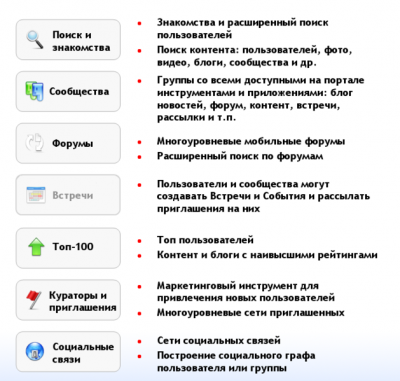
\includegraphics[scale=1]{sn-components.png} 
	\caption{Компоненты социальной сети}
	\label{fig:analysis:snComponents}
\end{figure}

Функции социальных сетей:
\begin{itemize}
	\item cоздание индивидуальных профилей, в которых будет содержаться определенная информация о пользователе;
	\item взаимодействие пользователей (посредством просмотра профилей друг друга, внутренней почты, комментариев и пр.);
	\item возможность достижения совместной цели путем кооперации (например, целью социальной сети может быть поиск новых друзей, ведение группового блога и пр.);
	\item обмен ресурсами (к примеру, ссылками на сайты);
	\item возможность удовлетворения потребностей за счет накопления ресурсов (например, путем участия в социальной сети можно обзаводиться новыми знакомыми и тем самым удовлетворять потребность в общении).
\end{itemize}

Классификация социальных сетей:
\begin{itemize}
	\item cоциальные сети в свободном доступе: не тематические сети и сугубо профессиональные сообщества практиков.
	\item cоциальные сети в корпоративном формате: cети в свободном доступе и не специализированные (сеть «общего профиля»).
\end{itemize}

Под не специализированными социальными сетями понимаются сообщества в интернете, не имеющие ограничений ни по каким параметрам и не имеющие никакой тематической специализации.

Специализированные социальные сети обычно являются платформой для сообществ специалистов. Они называются сообществами практиков (Community of Practice, CoP) и преследуют сугубо практические цели и объединяет людей, которые заинтересованы в приобретении и развитии знаний в определенной области, их использовании на практике. Сообщества практиков могут состоять из ученых, инженеров, специалистов по маркетингу и продажам и других специалистов. Причем эти сообщества не обязательно должны быть ограничены рамками одной компании, а могут объединять людей со схожими интересами в разных организациях по всему миру. CoP отличаются от сообществ по интересам — его участников объединяет не только стремление к некой области знаний, но и желание сотрудничать в процессе применения этих знаний на практике. Члены сообщества хорошо понимают друг друга, поскольку работают над схожими проблемами. Они способны оценить уровень квалификации, проблемы коллег, получить друг от друга недостающие им знания.

Социальные сети в корпоративном формате в первую очередь являются инструментом внутренних коммуникаций.
Т.к. темой дипломного проекта является создание тематической социальной сети -- разберем данный вид подробней.


